\newpage
\subsection{Pelican Drone}
In September of 2019, the Micro Air Vehicle Lab of Delft University of Technology released a brief blog post about their developed "pelican drone" \cite{pelicandrone}. The pelican drone is capable of taking water samples quickly and analyse them in a CytoSense, a device that scans algae and other micro organisms. Taking water samples by hand is quite expensive and labour intensive. A drone speeds up this process significantly, allowing for more samples at less cost. 

MAVLab claims the drone is fitted with a hyperspectral camera to detect harmful algae, though the video \cite{pelicandronevideo} shows no hyperspectral camera fitted on the drone or hyperspectral images taken from the drone.\\

Looking closer at the drone, it seems to be a first generation Swellpro SplashDrone Marine Warrior \cite{marinewarrior}, with its built-in payload release system used for mounting the rope with sample tube.

\begin{figure}[h]
  \centering
  \begin{minipage}[b]{0.4\textwidth}
    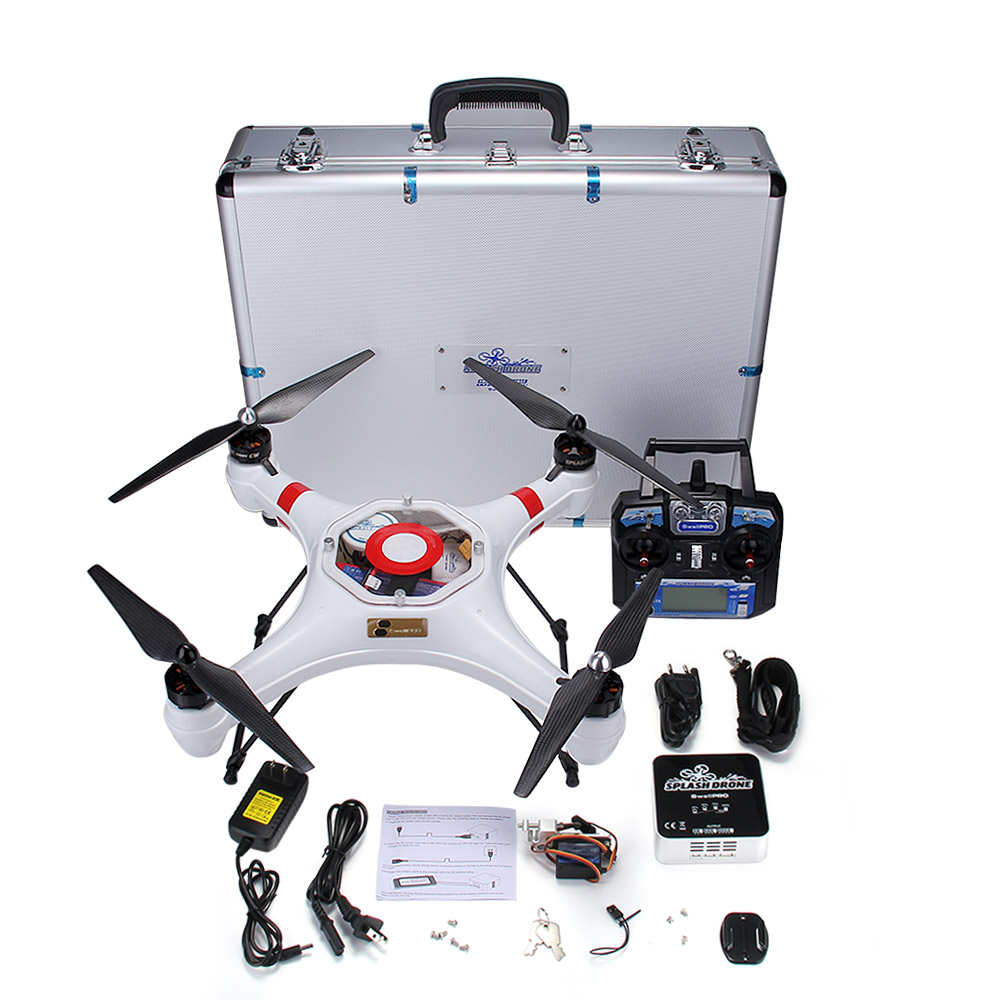
\includegraphics[width=\textwidth]{similarprojects/21_marinewarrior.jpg}
    \caption{Swellpro SplashDrone Marine Warrior \cite{marinewarrior}}
  \end{minipage}
  \hfill
  \begin{minipage}[b]{0.5\textwidth}
    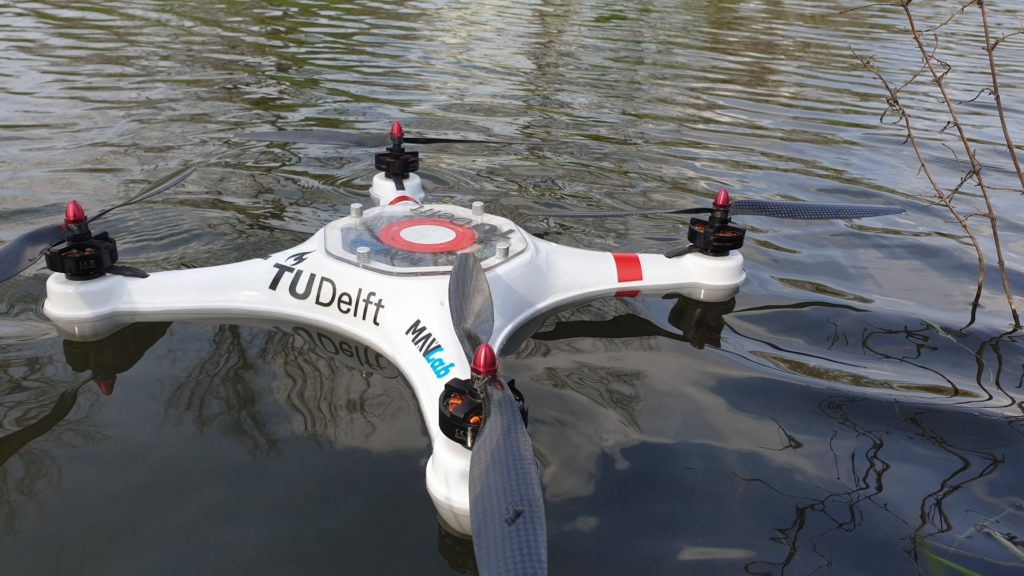
\includegraphics[width=\textwidth]{similarprojects/22_pelicandrone.jpg}
    \caption{TU Delft Pelican Drone \cite{pelicandrone}}
  \end{minipage}
\end{figure}

MAVLab states in the video and in the blog post that they were working on making the drone able to fly underwater.

Unfortunately, no further continuation of this project can be found. the initial blog post and video is all that is left. \cite{pelicandronevideo} 

\subsubsection{Similarity}
The pelican drone and this project both try to collect water samples using the drone. Where this project differs is that it also tries to measure multiple variables in real time using sensors.